\chapter*{Synthesis}
% Ajouter manuellement cette section à la table des matières
\addcontentsline{toc}{chapter}{Synthesis}

%   \usepackage{booktabs}   % pour \toprule \midrule \bottomrule
%   \usepackage{pgfplots}   % pour le graphique en barres
%   \pgfplotsset{compat=1.18}
%   \usepackage{xcolor}     % (déjà présent : couleur accenture)
%
% Le graphique est tracé nativement en pgfplots (pas d'image externe).
% ==============================================================

The principle of risk pooling is a cornerstone of insurance: it presupposes a relationship of trust between insurer and policyholder, which fraud diverts to illegitimate ends.

In non-life insurance, this phenomenon represents an estimated burden of around €2.5~billion per year in France, close to 5~\% of premium income, a significant part of which remains undetected. Beyond its direct cost, fraud adds around fifty euros to the premium of every honest policyholder on each motor contract and, over time, undermines the very solidarity of the mutualised pool.

The traditional fight against this phenomenon, based on the judgement of claims handlers and the intervention of specialised units, is now reaching its limits. It allows only a fraction of claims to be reviewed, depends heavily on the individual expertise of investigators, and comes up against an economic constraint that is difficult to overcome: the cost of a manual investigation makes it unprofitable to control low-value fraud, which is nonetheless the most widespread. It is from this observation that the present dissertation arose, its purpose being to present the step-by-step design and implementation of an automated motor-insurance fraud detection process, based on an artificial-intelligence agent and covering the entire chain, from data ingestion through to steering the system, such tools having already emerged on the market in recent years.

\bigskip

\noindent\textbf{Context and positioning:} The dissertation opens with a characterisation of insurance fraud, its typologies (opportunistic or organised, at underwriting or at the claim stage) and its legal framework, before establishing its economic stakes. The value of a detection system is not measured by its statistical performance alone, but by the claims burden it helps to avoid: this economic grounding, formalised through the notion of expected unit gain, constitutes the guiding thread of the work and justifies the fact that the choice of the model's parameters ultimately stems from a cost-benefit trade-off. The dissertation then provides an overview of detection methods, contrasting traditional manual approaches with the contributions of artificial intelligence, leading to a conviction that shapes the rest of the work: far from replacing human expertise, AI must be combined with it in a logic of complementarity, where the algorithm filters and prioritises while the human investigates and decides.

\bigskip

\noindent\textbf{Theoretical framework:} The methodological section presents the supervised models retained (from points-based scoring to logistic regression, through decision trees and ensemble methods such as Gradient Boosting), as well as the unsupervised approaches available for organised fraud (anomaly detection, clustering, graph analysis). Particular attention is paid to evaluation criteria suited to strong class imbalance: in a population where fraud is rare, standard indicators such as the overall accuracy rate become misleading, and should be replaced by the AUC-ROC, the Gini coefficient, the Kolmogorov-Smirnov statistic, precision, recall or the PR-AUC. This section finally stresses the requirements of governance, interpretability and regulatory compliance (GDPR, AI Act) framing the deployment of such models.

\bigskip

\noindent\textbf{Tool design:} The core of the dissertation is devoted to the concrete implementation of the motor-insurance fraud detection tool. The approach is deliberately confined to circumstantial fraud, detectable from structured data: claim characteristics, history of the policyholder and other parties involved, and consistency of the declaration. It draws on a public database of 30,000 motor claims and 24 variables, with a fraud rate of 11.5~\%. The database is then enriched with thirty additional variables, simulated by artificial intelligence, so as to reproduce the information actually available to an insurer (in particular the history of the repairer, the third party and the vehicle, declarative behaviour, and the geographical and temporal dimensions).

The tool is structured into two modules, corresponding to two clearly distinct user profiles as well as two usage timeframes. The first tool, intended for actuaries, handles the construction of the model: standardised data ingestion, automated auditing of data quality, descriptive statistical analyses, construction of the fraud prediction models and selection of the most performant model with respect to the defined quality criteria. The second tool, this time intended for claims handlers, exploits the previously calibrated model without exposing its complexity, nor even its inner workings: for each new claim entered, it returns a fraud probability and directs the handler towards a risk zone determining the level of investigation.

The logic used to build the agent is driven by a prompt broken down into successive steps, which reproduces the actuarial approach and guarantees the traceability of every link in the chain.

\noindent\textbf{Results:} The descriptive analysis brings out the major drivers of fraud: the central role of the repairer's environment, the policyholder's history of fraud, the consistency of the declaration, and the ratio between the repair invoice and the market price. A counter-intuitive finding emerges: fraud does not concern the most costly claims, which fully justifies the use of a multivariate approach. Three models are then built and compared along an interpretability-versus-performance trade-off, the results of which are summarised below.

\begin{table}[H]
    \centering
    \renewcommand{\arraystretch}{1.35}
    \begin{tabular}{l c c c}
        \toprule
        \textbf{Indicator} & \textbf{Points-based scoring} & \textbf{Decision tree} & \textbf{Gradient Boosting} \\
        \midrule
        AUC-ROC             & 0.923  & 0.838  & \textbf{0.942} \\
        Gini                & 0.846  & 0.676  & \textbf{0.885} \\
        KS                  & 0.688  & 0.565  & \textbf{0.740} \\
        Lift @10\,\%        & --     & $\times$4.61 & \textbf{$\times$6.66} \\
        PSI                 & 0.0008 & 0.0026 & 0.0023 \\
        Backtesting gap     & 0.009  & 0.039  & 0.026 \\
        \bottomrule
    \end{tabular}
    \caption{Summary of the quality indicators of the three models tested}
    \label{tab:synthesis-models}
\end{table}

Gradient Boosting stands out as the most discriminating model (AUC of 0.942, Gini of 0.885, top-decile lift of $\times$6.66) and is retained on that basis. The points-based \textit{scoring} model nevertheless remains a fully credible alternative: with an AUC of 0.923, it lies very close to Gradient Boosting while offering a transparency that ensemble methods do not allow, which makes it the preferred choice when explainability takes precedence. The decision tree, dominated on all criteria, is set aside. The three models moreover display excellent stability (PSI well below the alert threshold of 0.10) and good generalisation capacity.

One cross-cutting insight deserves to be highlighted: the three models, although built on different principles, converge in directing their explanatory power towards the same key variables, as illustrated by the profile of the retained model.

\begin{figure}[H]
    \centering
    \begin{tikzpicture}
        \begin{axis}[
            xbar,
            width=0.86\textwidth,
            height=8cm,
            xmin=0, xmax=30,
            xlabel={Relative importance (\%)},
            symbolic y coords={
                {Authorities contacted},
                {Nb of past claims (vehicle)},
                {Reporting delay},
                {Vehicle age},
                {Vehicle ownership duration},
                {Nb of amendments to the declaration},
                {Vehicle market value},
                {Nb of past frauds (policyholder)},
                {History of claimed amounts},
                {Invoice / market ratio (repairer)}
            },
            ytick=data,
            nodes near coords,
            nodes near coords align={horizontal},
            every node near coord/.append style={font=\footnotesize},
            bar width=9pt,
            enlarge y limits=0.08,
            tick label style={font=\footnotesize},
            label style={font=\small},
        ]
        \addplot[fill=accenture, draw=accenture] coordinates {
            (5,{Authorities contacted})
            (5,{Nb of past claims (vehicle)})
            (6,{Reporting delay})
            (6,{Vehicle age})
            (7,{Vehicle ownership duration})
            (8,{Nb of amendments to the declaration})
            (10,{Vehicle market value})
            (12,{Nb of past frauds (policyholder)})
            (16,{History of claimed amounts})
            (25,{Invoice / market ratio (repairer)})
        };
        \end{axis}
    \end{tikzpicture}
    \caption{Relative importance of variables in the retained model (Gradient Boosting)}
    \label{fig:importance-gb-en}
\end{figure}

\noindent\textbf{Deployment and governance:} Once the model has been selected and integrated, the tool is made available to the fraud detection department. On a day-to-day basis, the claims handler submits a claim, individually or in batches, and the tool returns for each one a fraud probability together with guidance on the investigation effort to undertake. Claims are thus sorted into three risk zones: a green zone (low probability, no investigation), an orange zone (intermediate probability, light investigation) and a red zone (high probability, in-depth investigation). The handler can therefore focus efforts on the highest-risk claims, without wasting time on those with a low probability of fraud.

\begin{figure}[H]
    \centering
    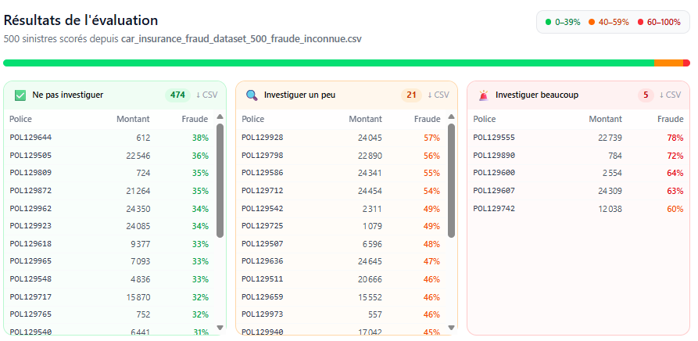
\includegraphics[width=0.95\textwidth]{images/chapitre6/tableau_proba.png}
    \caption{Evaluation results returned to the claims handler: scored claims sorted into three investigation zones (green / orange / red)}
    \label{fig:tableau-proba-en}
\end{figure}

The system is then completed by a continuous-enrichment feedback loop: once a claim's investigation is closed, its actual outcome (fraud confirmed or not) is recorded in binary form, and only claims thus qualified are added to the training database, allowing the model to recalibrate on established cases and to track the evolution of fraudulent behaviour over time. A monitoring report continuously restitutes the tool's added value through key indicators: the amount of fraud avoided thanks to the tool, the impact on the loss ratio (claims-to-premiums) and the return on investment (ROI). The whole framework remains under human oversight: the agent prioritises and directs claims, but issues no adverse decision automatically, the investigation and the final decision always resting with the investigator, in accordance with Article~22 of the GDPR and with the AI Act.

\bigskip

\noindent\textbf{Limitations and outlook:} The dissertation concludes with a critical reflection. Among the limitations are the partially simulated nature of the enrichment data, the likely over-representation of fraud in the database used (11.5~\% against around 5~\% in reality), and the need to recalibrate the model on a representative claims experience before any deployment. The tool nevertheless opens up many avenues for improvement: coupling with a policy database offering a historical and relational depth inaccessible at the level of the claim alone, the integration of external data, cross-insurer data pooling to detect "nomadic" fraudsters, or the extension to other non-life insurance lines. As the capabilities of artificial intelligence advance, the question is probably no longer whether these tools will transform the fight against fraud, but how insurers will manage to make use of them in a way that is at once performant, controlled and respectful of policyholders' rights.